\documentclass[12pt,a4paper,titlepage]{article}
\usepackage{fullpage}
\usepackage{hyperref}
\usepackage[pdftex]{graphicx}
\bibliographystyle{plain}
\newcommand{\HRule}{\rule{\linewidth}{0.5mm}}
\usepackage{url}
\usepackage{amsmath}
\usepackage{amsfonts}
\usepackage{enumitem}
\usepackage{float}
\usepackage{graphicx}
\usepackage{caption}
\usepackage{listings}
\usepackage{subcaption}
\usepackage{tabularx}
\usepackage[nottoc]{tocbibind}
\setlength{\parindent}{0.0in}
\setlength{\parskip}{0.1in}
\begin{document}
\renewcommand{\arraystretch}{1.9}
%\abovedisplayskip=2pt
%\abovedisplayshortskip=2pt
%\belowdisplayskip=2pt
%\belowdisplayshortskip=2pt
\begin{titlepage}
    \let\footnotesize\small
    \let\footnoterule\relax
    \let \footnote \thanks
    \setcounter{footnote}{0}
    \begin{center}
      \setlength{\parskip}{0pt}
       {\large School Of Electronics and Computer Science \par}
      {\large Faculty of Physical and Applied Sciences \par}
      {\large University of Southampton \par}
      \vspace{29mm}
      {\large Argyris Zardilis \par}	
	\vspace{4mm}
      \large \today
	\vspace{13mm}
        \center
        {\Large \bf Tool for parameter inference in dynamic biological systems \par}
        \vspace{60mm}
      {\large Project Supervisor: Dr. Srinandan Dasmahapatra \par }
      {\large Second Examiner: Dr. Markus Brede \par}
      \vspace{12mm}
        {\large A progress report submitted for the award of }\\
      {\large BSc Computer Science }
    \end{center}
    \vfil\null
  \end{titlepage}
\begin{abstract}
\nocite{gelman2003bayesian, Walsh04markovchain, lazebnik2002can}
Recent advances in experimental technology have given us detailed and comprehensive information on networks of biological interactions governing various functions of living organisms. This had led to an increase in the use of theoretical mathematical models to describe dynamic biological systems which has in turn led to an increasing need for computational tools to assist in the process of constructing these models and estimating their parameters from available experimental data. Although there is a rich literature on parameter estimation using a number of different techniques, very few attempts have been made to systematically attack the parameter estimation problem for these kinds of systems. From those, almost all of them attempt a mere reproduction of experimental data, disregarding important properties of those systems like their qualitative features and the effect of global system dynamics. 

In this study a computational tool has been produced tackling the parameter estimation problem in dynamic biological systems using different techniques and its success has been tested with real world models. Further to that, an attempt has been made to uncover the link and interplay between the practical considerations of the parameter inference process and the more theoretical tools of sensitivity and bifurcation analysis and therefore consequently to systems dynamics which are captured and understood through these. 
\end{abstract}
\tableofcontents
\newpage
\section{Introduction}
Cells of living organisms contain thousands of networks of biochemical interactions that perform their functions. Despite being, at the molecular level, subject to thermal noise and the random tinkering of evolutionary events they are able to perform their functions almost always without error and with remarkable consistency. The apparent high complexity of such networks has been perhaps one of the reasons that the main bulk of biological research has been focused on understanding the details of individual components instead of a systems-level understanding of their interactions. So in a way Biology did not follow the route of other natural sciences, like Physics for example, to try and find simplifying and general principles and laws that govern the behaviour of the natural systems occurring in living organisms using the theoretical framework of Mathematics. It might be because the general consensus was that living organisms are so complex and their behaviour is so highly stochastic at the molecular level that one will not be able to find these laws and express them using a rigorous language like Mathematics as used for inanimate objects. 

However recent advances in experimental technology like microarray experiments which enabled us to get the expression levels of a big number of genes at different time points have given us for the first time such detailed and comprehensive information on cellular processes.  Although the structure of such interactions has been assembled from the effects of many random evolutionary events over time, with this new volume of information we  are able to find common reoccurring network structures which evolution keeps turning to because exactly they are the ones that survive with their robustness. This leads us to think that they are common design principles behind these common network motifs that drive them so the goal of finding generalising and simplifying principles and gain systems level understanding through a theoretical framework inside the apparent complexity is revisited recently shifting some of the attention of biological research from experimentation to more theoretical work\cite{alon2007introduction}. Commonly occurring motifs (network structures) include switches, buzzers, blinkers\cite{tyson2003sniffers}, the inspiration for the decomposition and naming also coming from their resemblance to electronic-like components.

These common network motifs can then be assembled and be parts of larger networks of interactions that perform more complicated functions.  Such networks that their network structure is though to be well understood and have been the subject of much study both experimentally but even more theoretically include circadian oscillators and metabolic pathways\cite{bass2010circadian, sahar2012regulation, mirsky2009model}. As their name suggests one of the main properties of such networks of interactions is their structure, what are the interacting components and which one acts on what. The traditional way to capture this structure is with schematic means with the aid of a diagram an example of which can be seen in Figure \ref{fig:diagram_example}. Components of the networks are gene mRNA products and proteins which can either serve a biochemical function or act as transcription factors for genes. Transcription factors can act on genes to either activate:increase the rate of production or repress:decrease the rate of production of one or more genes. The gene products themselves though control the production of other proteins which can act as transcription factors(activators or repressors) to other genes or even themselves thus creating networks of interactions of varying complexity. The components of the network are the nodes of the diagram with their differences highlighted with the use of different shapes or colours while the interactions(regulations) are the edges differentiated by their ends; for example the flat end signifies repression while the arrow signifies activation. Several attempts to standardise these diagrams in the example of circuit diagrams in electronics (Molecular Interaction Maps\cite{kohn2006molecular}) have not been widely adopted so they still vary considerably across publications.
\begin{figure}
\centering
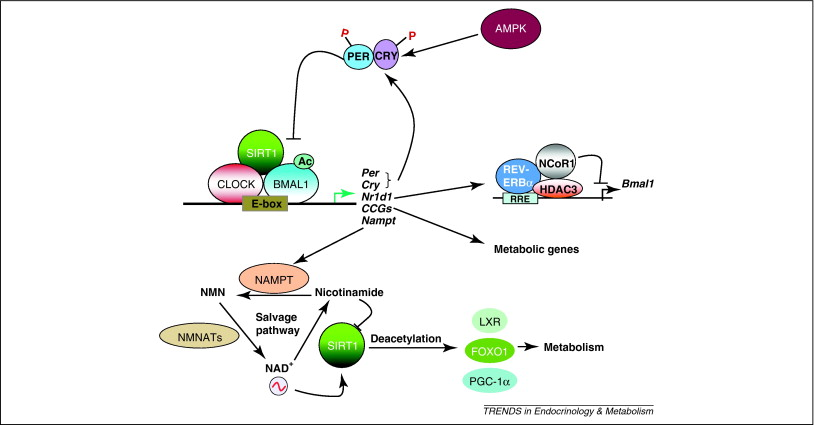
\includegraphics[width=0.9\linewidth]{clock_metabolism}
\caption{Networks of interactions between circadian clock and metabolic pathways\cite{sahar2012regulation}}

\label{fig:diagram_example}
\end{figure}

The network structure, though important, is only one of the properties that help us get insight into the workings of these systems. Another essential property which becomes even more apparent as the diagrams and networks grow in size is the systems dynamics. The diagrammatic way of describing the systems is very poor in that sense as it does not capture the dynamic properties that these systems exhibit\cite{kitano2002computational}. The natural way to capture the dynamic behaviour of systems that is being used throughout science is with differential equations. That way we can use a more theoretical and well researched framework of Mathematics and of dynamical systems in particular  to talk about these systems and borrow tools from it that aid the analysis process and give us greater insight to eventually build a systems-level understanding of complex biological systems. %write something about the further goal, synthetic biology durg design etc.
The we can ask more complicated and interesting questions like: what are the control mechanisms that drive these systems? how does one part affect others? Which parts provide the stability and robustness to the system? How will the system behave in the future with the same or varying conditions? The diagrams which offer the static structure provide very little knowledge and surely cannot answer these questions.

Systems can be thought of as stochastic processes as they are subject to molecular noise and various fluctuations in their interactions. Therefore they can be expressed as stochastic differential equations or their evolution can be simulated with the Gillespie algorithm\cite{gillespie1977exact} or one of its more recent variants\cite{gillespie2001approximate, gibson2000efficient}. However the effects of these fluctuations are only considerable when the number of molecules of the reactants is very small so more often the average case is considered and the systems are expressed as deterministic Ordinary Differential Equations(ODEs) like so: 
\begin{equation*}
\mathbf{\dot x} = \mathbf{F}(\mathbf{x}, t, \mathbf{\theta})
\end{equation*}
 These describe the evolution in the concentrations of components of the systems(variables) over time and are parameterised by $\mathbf{\theta}$ which mainly describes the kinetic rates of the reactions/regulation or other constants like initial concentrations. So the evolution of the concentration of component $x1$ might be described by $f(\mathbf{x}, t, \theta)$ which tells us how the concentration is altered through the effects of other variables(components) or itself over time. These equations are translations of the diagrams and the duality of the representation can be seen through an example. Let's consider the a simple synthetic network motif seen in Figure\ref{fig:simple_motif}. 
\begin{figure}
\centering
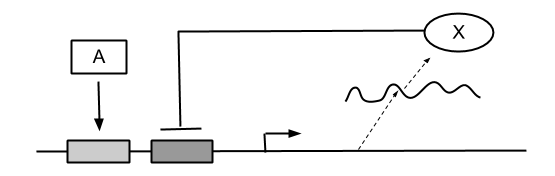
\includegraphics[width=0.5\linewidth]{neg_autoregulation}
\caption{Negative autoregulation network motif: Gene X and its protein product are regulated by A. Protein product X also represses its own production\cite{alon2007introduction}(chapter 1)}
\label{fig:simple_motif}
\end{figure}
This is a common negative autoregulation motif which occurs in 40\% of known transcription factors in E.Coli\cite{rosenfeld2002negative}. In this network gene X(and its protein product) is regulated by A. The protein X acts as a transcription factor for its own gene repressing its own production. We are concerned with the concentration of protein product X so that is one of our variables. Now we need to express the change in its concentration as an equation. The production of protein X is balanced by the dilution due to the growing area of the cell and the degradation due to its natural destruction. Therefore the change in the concentration can be expressed as the difference between the two processes(production and dilution/degradation).  The regulation of X by A(transcription and translation) is orders of magnitude faster than the change in the concentration of X so we can assume the production rate due to A's regulation is constant at a rate $\beta$. However the production rate is also affected negatively by X itself so it should be a decreasing function of X with $\beta$ as its maximum value when $X=0$. One such function that is found to agree with observation is the Hill function: $ f(X) = \frac{\beta}{1 + \left(\frac{X}{K}\right)^n}$. The dilution/degradation process at a rate $\alpha$ is proportional to its concentration so the resulting differential equation for the concentration of X is:
\begin{equation}
\frac{dX}{dt} = \frac{\beta}{1 + \left(\frac{X}{K}\right)^n} - \alpha X
\label{eq:neg_autoregulation}
\end{equation}
The Hill equation for the repressor can be derived from simple chemical kinetic laws like the law of mass-action\cite{} or Michaelis-Menten kinetics\cite{}(see Appendix A in \cite{alon2007introduction} for a detailed derivation and explanation). Starting from these simple laws one can describe as equations all reactions and therefore all systems. The intuition and background knowledge of the modeler though is needed for simplifying the models, for example as we have done for the transcription factor A where we treated it as constant due the differences in timescales between the processes(Quasi-steady-state approximation). 

For this simple model, one could easily understand the dynamics of it just by looking at it. However for most systems this is not very easy and most of these systems cannot be solved analytically. This is where the knowledge from the field of dynamical systems comes in. One of the main observations and driving force in field of dynamical systems is: we cannot solve these systems analytically so how can we understand their dynamic behaviour from the differential equations themselves. Of course now we can solve these systems numerically and get  good idea of how these systems evolve over time. To solve numerically though we need values for the parameter quantities like $\beta, K, n, \alpha$ in Eq\ref{eq:neg_autoregulation}. These parameters in these models have a physical interpretation: production/degradation rates, binding affinities, transport rates, etc. This generally poses an issue because quantitative data on these parameters are rarely available because they are difficult to measure experimentally. 

The problem therefore is to estimate those parameter values from experimental measurements of the concentrations of the network components over a time period, data which might be scarce or incomplete. This problem sometimes called the inverse problem can be seen as going from the real world observables to the mathematical models that represent those observables. Doing that for parametric models is equivalent to finding the parameters. This inverse problem is a common theme in Machine Learning so there is a large toolbox of available techniques to tackle the problem. However these classical methods are not always suited to such complex systems and might fail. Moreover there are more factors that come into play as far as biological systems are concerned which are not captured by these techniques. The increase in the available computational power has made possible the introduction of new techniques which are based on simulation which have been shown to be more suited to the task. However there have been very few attempts to produce computational tools that aid in the modeling process and attack this problem in this domain despite its importance(see \ref{sec:background} for a more detailed treaty on parameter estimation methods used in this domain and relevant tools). It is with this inference problem and these new techniques that this study is concerned with.  The first part of this project has been to use these new techniques to produce a computational tool that automatically and systematically attacks the parameter estimation problem. Discussion and results are covered in chapter 1 of this study. 

\begin{figure}
\centering
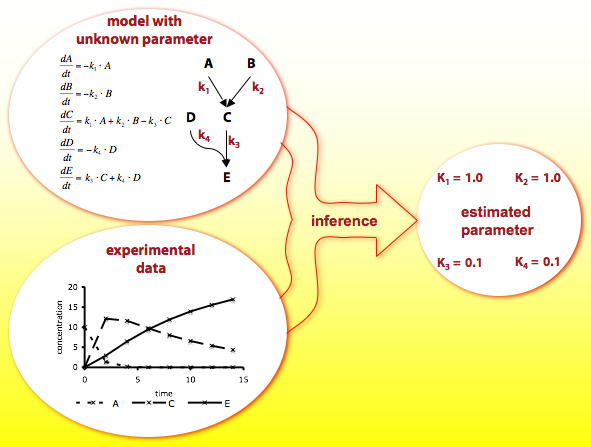
\includegraphics[width=0.5\linewidth]{inference}
\caption{Parameter inference methods combine experimental data with the knowledge about the underlying structure of a dynamical system to be investigated. Unknown model parameter (here k1, k2, k3 and k4) can be estimated.}
\label{fig:inference}
\end{figure}

Work on the first task of this project has led to some observations that potentially link the parameter estimation procedure with some more theoretical tools and aspects of the systems in question.  
As has been previously discussed systems dynamics play an important role in our understanding of complex biological systems. The language of choice for their description(differential equations) enables us to use some of the tools developed in the field of dynamical systems to investigate the dynamics. Simple models like the one for the negative auto-regulation network motif described previously are easy to understand intuitively but as the models grow intuition alone cannot help. Sensitivity analysis on these models tells us how much the observable behaviour of the system depends on specific parameters of the model. The second part of this study is firstly concerned with the connection between the practical considerations of parameter estimation and the more theoretical tool of sensitivity analysis. Is there a connection between the estimate for a parameter and the model's sensitivity to it? Bifurcation is a change in a system's dynamics as one of its parameters passes through a bifurcation point. In parameter estimation the effects of global dynamics are hardly ever considered despite the fact that their importance in understanding biological systems has been demonstrated\cite{}. Do these global dynamics affect the parameter estimation procedure? This is also something that we try to address in the second part of this study.


%=======================================================================================================================================================================================================================
%=======================================================================================================================================================================================================================
%=======================================================================================================================================================================================================================


\section{Background Research}
\label{sec:background}
The parameter estimation problem as posed in the previous section is the inverse problem of going from world observables to models that represent those observables. To formalise this problem, we have a proposed model for our system which describes the evolution of all variables(components) $\mathbf{x} = \{x_1, x_2, \dots, x_n\}$,
\begin{equation}
\label{eq:system}
\begin{array}{lcl}
\dot x_1 & = & f(\mathbf{x}, t, \theta) \\
\dot x_2& = & f(\mathbf{x}, t, \theta) \\
\vdots \\
\dot x_n & = & f(\mathbf{x}, t, \theta), \\
\end{array}
\end{equation}
We also have the observations of the world in the form of experimental data at $N$ different time points, $\mathbf{Y_d} = \{\mathbf{y}_{t_{1}},  \mathbf{y}_{t_{2}}, \dots, \mathbf{y}_{t_{N}}\}$ where the observation at time point $t_{k}$ is the state of the system(concentration of $n$ variables) at that point so 
$\mathbf{y}_{t_{k}} =\{ x_{1}^{t_{k}},  x_{2}^{t_{k}}, \dots,  x_{n}^{t_{k}} \}$. The problem then become to find the parameter vector $\theta^*$ from the set of all the possible parameter vectors $\mathbf{\Theta}$ so that the model $\mathbf{\dot x} = \mathbf{F}(\mathbf{x}, t, \mathbf{\theta^*})$  \ref{eq:system} fits the experimental data best. The fitness of a particular parameter vector $\theta_{s}$ can be assessed with a distance metric between the experimental data $\mathbf{Y}_{d}$ and a simulated solution $\mathbf{Y}_{s}$ for proposed parameter $\theta_{s}$. Then the problem becomes the minimisation of this distance metric and this is the common optimisation problem formulation: 
\begin{equation*}
\theta^* = \underset{\theta}{\arg\min}(\Delta(\mathbf{Y_{d}},\mathbf{Y}_{\theta})) 
\end{equation*}
where $\Delta$ is some distance metric, also called cost or objective function in optimisation language. Naturally much attention has been given on parameter estimation for deterministic systems with local and global optimisation methods\cite{Moles2003param}.  Generally optimisation algorithms have the same outline:
\begin{enumerate}[noitemsep]
\item{Start with some choice $\theta_{s}$ for model's adjustable parameters from $\mathbf{\Theta}$}
\item{Simulate solution $\mathbf{Y}_{s}$ for proposed parameter $\theta_{s}$ and evaluate distance/cost function}
\item{Stop if some termination criterion is met, for example cost function is less than some threshold value $\epsilon$}
\item{Generate a new guess $\theta_{s}$ from $\mathbf{\Theta}$}
\item{Return to 2}
\end{enumerate}
Then the difference between different choices for optimisation algorithms is how to more efficiently search the parameter space $\mathbf{\Theta}$ and all the classic techniques like steepest-descent, variants of Newton's method, Levenberg-Marquardt have been used in different applications with varying degrees of success\cite{mendes1998non}. Other optimisation techniques used in some application include simulated annealing\cite{kirkpatrick1983optimization} which makes stochastic decisions for the movement in the search space $\mathbf{\Theta}$ to avoid common problems of classic optimisation algorithms like getting stuck at local extrema. Attempts to compare different optimisation techniques generally come to the conclusion that the success of the algorithm depends on the application and that there is no single algorithm that outperforms the others in all applications while there is also the risk that some algorithms that perform well in some problems might even fail completely in others(for a full treatment and comparison of a number of different methods see \cite{mendes1998non}). 

A maximum-likelihood approach to parameter estimation in this domain has also been used for some applications. In this formulation of the problem, one tries to find the values of the parameters that are more likely to have been used to generate the observed data in other words trying the maximise the likelihood function of the data given the parameters. Likelihood functions are generally associated with probabilistic models and Maximum Likelihood Estimation(MLE) with information-theoretic approaches but subject to some assumptions MLE reduces to traditional least-square data fitting,
\begin{itemize}[noitemsep]
\item{The observational errors are normally distributed}
\item{Equivalent positive and negative deviations from the expected values differ by equal amounts}
\item{The errors between samples are independent.}
\end{itemize}
(We will use these assumptions later in the chapter 2 to plot and investigate the shape of the likelihood functions under different values of the bifurcation parameter for different models). The models generally involve non-linear combination of the parameters so the least-squares formulated problem has no closed form solution. Then one has to resort to numerical optimisation techniques like the ones outlined in the previous paragraph. These general optimisation routines are commonly available in many packages for many programming languages and popular programming environments for scientific computation like \href{http://www.mathworks.co.uk/products/optimization/}{MATLAB} , \href{http://www.gnu.org/software/octave/doc/interpreter/Optimization.html}{Octave}, \href{http://docs.scipy.org/doc/scipy/reference/tutorial/optimize.html}{scipy(Python)}.

In population genetics applications Approximate Bayesian Computation(we will to refer to them as ABC from now on) in its most basic rejection sampling form has been used\cite{pritchard1999population}. The traditional Bayesian formulation of the problem is to try to find the posterior distribution of the parameters $\theta$ given data $\mathbf{Y}_{d}$, $\pi(\theta | \mathbf{Y}_{d})$ given in this setting by $\pi(\theta | \mathbf{Y}_{d}) = L(\theta)\pi(\theta)$ where $L(\theta)$ is the likelihood function and $\pi(\theta)$ is the prior distribution of the parameters. ABC methods use a simulation-based procedure to eliminate the computation of the likelihood function in cases where it is intractable or impossible to do so. Other forms of ABC which build and improved on the same idea include Markov Chain Monte Carlo methods\cite{marjoram2003markov} and different variants of Sequential Monte Carlo\cite{del2006sequential, sisson2007sequential, toni2009abc}. These became more popular recently due to the increase in computational power and that can be seen by the amount of recent publications. It is with these different forms of these ABC methods that we will be concerned with in this study. These methods have been shown to work without considerable modification in a diverse range of applications\cite{toni2009abc} and also provide richer information which can be used to get some insight into some aspects of the dynamical systems in question as we will do in the second part of this report.

One of the problems with these numerical approaches is that they disregard qualitative features of the models that are equally if not more important than quantitative and exact replication of experimental data. Some qualitative feature which their importance has been discussed and that do not show up in the numeric data include specific phase-response curves for circadian oscillators\cite{pfeuty2011robust}%probable need to add another example here!
There have been a few attempts to capture some qualitative features like the shape of the data for model selection purposes. They rely on comparisons of the Fourier Transform of the original dataset and simulated dataset to select the model that best fits\cite{konopka2010gene}. We use this comparison between Fourier Transforms as part of the distance function we use for the comparison of original and simulated dataset in the ABC implementations with various degrees of success.

So there is a wide variety of techniques available to use in the problem but as far as application tools go the choice is not that big. There are a few tools (\href{http://www.math.pitt.edu/~bard/xpp/xpp.html}{XPP-Auto}, GRIND, \href{http://www.copasi.org/tiki-view_articles.php}{COPASI}) that are used because they allow modelers to get an intuition and greater understanding of the model in question usually by graphical means such as plotting bifurcation diagrams and allowing them to see the changes in the dynamics of the system as parameters change. And although they help in parameter estimation they do not address the problem directly. One tool that addresses the problem directly is the ABC-Sysbio\cite{liebe2010abcpy} which can be embedded in external code or used as a stand-alone application. This tool does automatic parameter estimation using Sequential Monte Carlo method.


%=======================================================================================================================================================================================================================
%=======================================================================================================================================================================================================================
%=======================================================================================================================================================================================================================


\section{Parameter Estimation}


In this study we have mainly focused on ABC methods as outlined in the previous section. The use of ABC methods arose in applications where the computation of the likelihood function,
\begin{equation*}
L(\theta) = f(\mathbf{Y_{d}} | \theta),
\end{equation*}
where $\mathbf{Y_{d}}$ are realisations of the data and $\theta$ is the parameter vector associated with the model, is impossible or impractical. The main theme in ABC approaches is the use of systematic comparisons between real data and simulated data to approximate the Likelihood function and therefore arrive at the desired posterior distribution,
\begin{equation*}
p(\theta|\mathbf{Y_{d}}) \propto f(\mathbf{Y_{d}|\theta})\pi(\theta),
\end{equation*}
where $\pi(\theta)$ is the prior distribution of parameters $\theta$. Typically simulating from $f(\mathbf{Y_{d}} | \theta)$ is straightforward. We then compare the simulated dataset $\mathbf{Y_{s}}$ with the real data $\mathbf{Y_{d}}$ and accept only those simulations where some distance metric between the two $\Delta(\mathbf{Y_{s}}, \mathbf{Y_{d}})$ falls below a certain threshold value $\epsilon$.  Generally ABC methods have the following form:\begin{enumerate}[noitemsep]
\item{Sample a parameter vector $\theta^*$ from a proposal distribution $\pi(\theta) $}
\item{Simulate a dataset $\mathbf{Y_{s}}$ from the model characterised by conditional probability distribution $f(\mathbf{Y_{d}}|\theta)$}
\item{Compare the simulated dataset $\mathbf{Y_{s}}$ and observations $\mathbf{Y_{d}}$ according to some distance function $\mathrm{\Delta}$. If $\Delta(\mathbf{Y_{s}}, \mathbf{Y_{d}}) < \epsilon$ where $\epsilon$ is the error tolerance of accepted solutions, then accept $\theta*$ otherwise reject. }
\end{enumerate}
The output of the ABC algorithm is a sample from a distribution of the form,
\begin{equation}
p_\epsilon(\theta|\mathbf{Y_{d}}) \propto \int f(\mathbf{Y_{s}}|\theta)  (\Delta(\mathbf{Y_{d}}, \mathbf{Y_{s}} \leq \epsilon) \pi(\theta)  \text{ }\mathrm{d}\mathbf{Y_{s}},
\end{equation}
If the chosen value for $\epsilon$ is small enough then the obtained distribution $p_\epsilon(\theta | \mathbf{Y_{d}})$ will be a good approximation for $p(\theta | \mathbf{Y_{d}})$. Sometimes when the comparison between real and simulated datasets is difficult summary statistics of the datasets, $S(\mathbf{Y_{d}})$ and $S(\mathbf{Y_{s}})$ can be compared instead. The ABC scheme as outlined above is not very efficient in its search of the parameters space as it spends a lot of time in areas of very low likelihood where the simulated solution will no resemble the data. To this direction different computational schemes have been devised like Markov Chain Monte Carlo\cite{marjoram2003markov} where previous good choices advise the next choices thus creating a Markov Chain with stationary distribution the posterior and Sequential Monte Carlo methods where you sample with a decreasing $\epsilon$-schedule and from a series of distributions that increasingly resemble the target posterior\cite{del2006sequential, sisson2007sequential, toni2009abc}. These are the basic flavours of ABC methods although there are variants of each and these were the methods implemented and incorporated for the parameter estimation tool. In the next section there are more detailed accounts for the implemented algorithms followed by test results on 2 systems.

\subsection{Simple Rejection Sampler}
\label{sec:rejection_sampler}
The simpler ABC algorithm is a simple rejection sampler\cite{pritchard1999population} which basically follows the general form as outlined before without any modifications. It samples from a prior distribution without taking into account correct guesses and 'blindly' continues to draw samples from the prior:
\begin{enumerate}[noitemsep]
\item{Sample a parameter $\theta ^*$ from prior distribution $\pi(\theta)$.}
\item{Simulate a dataset $\mathbf{y}^*$  from model with parameters $\theta ^*$.}
\item{If $\Delta(\mathbf{Y_{s}}, \mathbf{Y}) < \epsilon$ accept $\theta^*$, otherwise reject.}
\end{enumerate}
The distance function used is a simple Euclidean distance metric,
\begin{equation}
\sum_{i=0}^{N} (\mathbf{Y_{d}}^{i} -\mathbf{Y_{s}}^{i})^2,
\end{equation}
where $\mathbf{Y_{s}}$ is the simulated dataset and $\mathbf{Y_{d}}$ is the observed dataset. This distance metric is related to traditional Maximum Likelihood Estimation subject to some assumptions and we will show that in detail in a later section. Obviously the acceptance rate for this algorithm is really low if the prior distribution is very different from the posterior since it does not take into account previous good guesses to inform the search and keeps 'blindly' jumping in parameter space. This low acceptance rate means a high number of simulation steps are needed to get a reasonable number of accepted samples to approximate the posterior and although the simulation does not have a high computational cost the number of steps needed make this algorithm a poor choice and it was just implemented as a reference point to see the improvements with the more sophisticated algorithms. For precise results see later section.
\subsection{Markov Chain Monte Carlo(MCMC)}
An improvement to the random search of the simple rejection sampler is offered by a Markov Chain Monte Carlo method in the spirit of the traditional Metropolis-Hastings algorithm but slightly modified to fit this problem\cite{marjoram2003markov}. The intuition behind this algorithm is that you use previous good guesses as a basis for the next sampling thereby creating a Markov Chain with stationary distribution the goal posterior:
\begin{enumerate}[noitemsep]
\item{Initialise $\theta_{i}, i = 0$.}
\item{Sample a candidate parameter vector $\theta^*$ from a proposal distribution $q(\theta^* | \theta_{i})$.}
\item{Simulate a dataset $\mathbf{y}^*$ from model with parameters $\theta^*$.}
\item{If $d(\mathbf{y}^*, \mathbf{Y}) < \epsilon$ jump to new value $\theta^*$ - making it the next value in the chain, $\theta_{i+1} = \theta^*$- with a probability given by:
\begin{equation*}
a = min \left(1, \frac{\pi(\theta^*)q(\theta_{i} | \theta^*)}{\pi(\theta_{i}q(\theta^*|\theta_{i})}\right)
\end{equation*}}
\item{Set i=i+1 and continue from 2.}
\end{enumerate}
One of the decisions that was taken was to use an adaptive Gaussian distribution as a proposal distribution $q$. The proposal Gaussian from which we sample has big variance at first so that it will make big jumps in the parameter space. Once a good sample is found the variance of the proposal distribution is decreased to stay in the area. But that has the problem of getting stuck at local optimum areas for a long period of time so a rejection count is employed. If in the close vicinity we keep rejecting then the variance of the proposal distribution is increased to move out of that area. That way areas with many accepted samples are oversampled in the final population. It should be noted that univariate Gaussians were used for the proposal distributions, with each parameter in the parameter vector $\theta$ coming from a different proposal distribution. The relations between the parameters are however captured in the fact that when a sample is accepted it is accepted as whole. Despite the attempts to avoid the problem of getting stuck at local sub-optima, this algorithm is still prone to doing exactly that. One possible improvement is to change it to the original Metropolis-Hastings and therefore accepting (with low probability) samples that do not come close to the observed data. That way sometimes jumps will be made to other areas which can result in better exploration of the parameter space. This can also give a resulting population with more than one candidate value and then other criteria can be used to evaluate the fitness of the model with both set of candidate parameters. 
\subsection{Sequential Monte Carlo(SMC)}
Another variation of the ABC form is the Sequential Monte Carlo approach\cite{toni2009abc} which combines the common ABC algorithm form with a Sequential Monte Carlo approach.  In this algorithm instead of having a single $\epsilon$ value as tolerance we have an $\epsilon$ schedule of a series of decreasing values $\epsilon_T < \epsilon_{T-1} \dots < \epsilon_{1}$. We start by sampling from the prior $\pi(\theta)$ as before at algorithmic time $t=1$ with a tolerance level $\epsilon_{1}$. Then we accept or reject the generated samples with a comparison between real and simulated data in the standard ABC fashion. The population of accepted particles is therefore an approximation for $p_{\epsilon_{1}}(\mathbf{Y_{d}}|\theta)$. Then at algorithmic time $t=2$ instead of sampling again from the prior $\pi(\theta)$ we sample from the distribution obtained at the previous step $p_{\epsilon_{1}}(\mathbf{Y_{d}}|\theta)$. The new samples are perturbed with a perturbation kernel. The perturbed particles are then accepted or rejected as before subject to new tolerance level $\epsilon_{2}$ thus creating the second population. This procedure is repeated for all all $T$ tolerance levels in the $\epsilon$-schedule therefore creating distributions \{$p_{\epsilon_{1}}(\mathbf{Y_{d}}|\theta)$,$p_{\epsilon_{2}}(\mathbf{Y_{d}}|\theta), $\dots, $p_{\epsilon_{T}}(\mathbf{Y_{d}}|\theta)$\} along the way. If the final $\epsilon_{T}$ is small enough then the final population should be a good approximation of the target posterior.  The algorithm therefore describes a particle-filtering procedure -we pass and filter a population of parameter values sampled from a prior $\pi(\theta)$  from a series of distributions with the decreasing $\epsilon$-schedule so that the intermediate distributions gradually go towards the posterior(this particle-filtering view can be better seen with Figure\ref{fig:smc}). The particular SMC algorithm that we use is from \cite{toni2009abc} which also uses the notion of importance sampling, assigning weights to each particle in the population and then in the next step sampling from the weighted distribution,
\begin{figure}
\centering
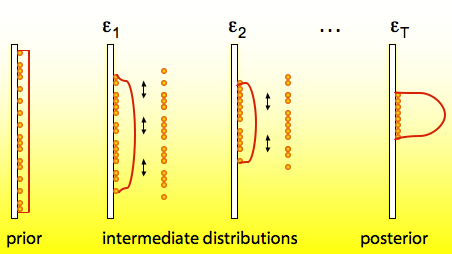
\includegraphics[width=0.5\linewidth]{ABCSMC}
\caption{In the SMC algorithm a sample from the prior distribution $\pi(\theta)$ is passed through filtering steps where the probability of the particles to represent the data best is updated during the algorithm via intermediate distributions. The final distribution $p_{\epsilon_{T}}$ is an approximation of the posterior distribution. The SMC  algorithm follows a particle-filtering approach.}
\label{fig:smc}
\end{figure}

\begin{enumerate}[noitemsep]
\item{Initialise the $\epsilon$-sequence $\epsilon_{1}, \dots, \epsilon_{T}$}
\item{If $t=0$, sample $\theta^**$ from prior $\pi(\theta)$\\
Else, sample $\theta^*$ from previous population $\theta_{t-1}^{i}$ with weights $w_{t-1}$ and perturb it with a perturbation kernel $K_{t}(\theta|\theta^*) $ to get particle $\theta^{**}$.}
\item{Simulate dataset $\mathbf{y}^*$ from model with parameters $\theta^{**}$.}
\item{if $d(\mathbf{y}^*, \mathbf{Y}) > \epsilon_{t}$ go back to 2, otherwise accept particle -set $\theta_{t}^{(i)} = \theta^{**}$- and calculate its associated weight by:
\begin{equation*}
w_{t}^{(i)} = \begin{cases} 1, & \mbox{if } t\mbox{ = 0} \\ \frac{\pi(\theta_{t}^{(i)})}{\sum_{j-1}^N w_{t-1}^{(j)}K_{t}(\theta_{t-1}^{(j)}, \theta_{t}^{(i)}} , & \mbox{if } \mbox{$ t > 0$} \end{cases}
\end{equation*} }
\item{Continue for all $\epsilon \in \left\{{\epsilon_{1}, \dots, \epsilon_{T}}\right\}$}
\end{enumerate}

It should be noted that in the special case where $T=1$ the algorithm reduces to the simple rejection algorithm described in section \ref{sec:rejection_sampler}.  The success of the algorithm both in computational and quality of the solution depends on the choice of the $\epsilon$ schedule and the perturbation kernel $K_{t}$. The effect of the $\epsilon$-schedule is easy to see: if two successive tolerance levels $\epsilon_{t}$ and $\epsilon_{t+1}$ are close to each other then the corresponding intermediate distributions $p_{\epsilon_{t}}(\mathbf{Y_{d}}|\theta)$ and $p_{\epsilon_{t+1}}(\mathbf{Y_{d}}|\theta)$  will be similar and therefore the acceptance rate of the filtering procedure at that step will be high with the disadvantage however that the procedure will not much progress towards the posterior.  A slowly decreasing $\epsilon$-schedule will therefore results in a high number of filtering steps(large value of $T$). On the other hand if two successive tolerance values are further apart the opposite holds: the acceptance rate will suffer but the progress of the algorithm will be faster with a lower number of iterations. Despite the easy to understand intuition determining what tolerance values are close and which ones are not depends on the application at hand. Therefore there is the danger that the algorithms completely fails with particular choices of the $\epsilon$-schedule. The common choice until recently was to manually fix the schedule of tolerance values beforehand according to the model however there have been proposals for an adaptive schedule. Although we started with a hand-tuned schedule we changed that to an adaptive choice. At step $t+1$ the choice for the tolerance level, $\epsilon_{t+1}$ at that step is based on the $a$-th quantile of the distances between the accepted simulated data $\{\mathbf{Y_{s}}^{(i,t)}\}_{1 \le i \le N}$ and real data $\mathbf{Y_{d}}$ at previous step $t$. We have found that the adaptive choice for the schedule with the correct choice of $a$ improves the efficiency of the algorithm significantly for our tests cases. However in \cite{silk2012optimizing} it is argued that some choices of $a$ may result in the algorithm not converging to the required posterior $p_{\epsilon}(\cdot| \theta)$ so the value of the choice of the quantile is an important one.

The second algorithm setting that affects the performance is the choice for the perturbation kernel $K_{t}$. A local perturbation kernel hardly moves the particles and therefore results in high acceptance rates in the filtering steps if the successive tolerance levels are close enough.  A perturbation kernel with higher variance spreads the search more resulting in better exploration of the parameter space but at the cost of low acceptance rates. Various perturbation kernels have been proposed, component-wise normal and uniform, multivariate normal and uniform, more local ones depending on a part of the previous population or on the local Fisher Information. In \cite{filippi2011optimal} they also try to find optimality criteria for these kernels. In our implementation at first a component-wise perturbation uniform kernel was used so each parameter was sampled and perturbed independently. The $k$-th component of parameter vector $\theta$ was perturbed with uniform kernel $\sim \mathcal{U}(\theta_{k}-\sigma_{j}^{t}, \theta_{k}+\sigma_{j}^{t})$.  We set the value for $\sigma_{j}^{t}$ to the scale of the previous population,
\begin{equation*}
\sigma_{j}^{t} \approx ( \underset{1 \le j \le N}{\max}\{\theta_{k}^{t-1}\} - \underset{1 \le j \le N}{\min}\{\theta_{k}^{t-1}\}).
\end{equation*} 
We have also tried multivariate kernels and in particular one with M-nearest neighbours.  This proceeds in the following way:  for each sampled particle $\theta$ its M nearest neighbours from the previous population $\{ \theta^{(\i, t-1)}m 1 \le i \le N\}$ are selected and the particle is perturbed according to a multivariate Gaussian distribution with mean $\theta$ and covariance matrix the empirical covariance matrix of those M-nearest neighbours, $\Sigma_{\theta, M}^{(t)}$.  

We provide some results in the Results section\ref{sec:results} in an attempt to compare the efficiency between the different settings of the algorithm but for a more detailed and formal treaty of the topic we refer to \cite{filippi2011optimal}. 
\subsubsection{Using Fourier Distance as a distance metric}
In the work of \cite{konopka2010gene}, the observations for the system's variables are treated as signals and their Fourier Transforms are used as a tool for model selection. We try to use the Fourier Transform as part of the distance function $\Delta$ that is used to compare real and simulated data in the SMC algorithms in order to try and capture some qualitative features of the system in question like the shape of the functions.For example this is particularly important for applications that require the presence of oscillations. In those cases a mere reproduction of the experimental data is not enough. We created a new value called 'Fourier Distance' between real $\mathbf{Y_{d}}$ and simulated datasets $\mathbf{Y_{s}}$ defined as the average distance between the dominant components of the Fourier Transforms of the constituent signals(variables) of the two.

%get results with different kernels adaptive schedule etc.
\subsection{Results}
In this section we will test the implemented algorithms on two models. For the first model we will focus on the differences between ABC flavours, rejection sampling, MCMC, SMC. For the second model we will only test the SMC algorithm and focus on the differences between different settings of the algorithm namely the choice for $\epsilon$-schedule and perturbation kernel. The second model is also chosen purposefully to illustrate some of the richness of information obtained from the SMC algorithm regarding system's dynamics and sensitivity.

\subsubsection{Parameter inference for the Lotka-Volterra model}
The algorithms were first tested on the simple Lotka-Volterra predator-prey system\cite{lotka1925elements}. It is a well studied system which consists of two coupled non-linear differential equations which correspond in the original interpretation to populations of predators and prey, 
\begin{equation}
\begin{array}{lcl}
\dot x &=& ax - xy \\
\dot y &=& bxy - y \\
\end{array}
\end{equation}
The system has two fixed points at $(0, 0)$ and $(a, 1/b)$. We are interested in the second fixed point because closed trajectories surround it in phase space corresponding to solutions which oscillate around that fixed point. We set the parameter values $(a,b) = (1,1)$ which make the second fixed point $(1, 1)$ so we set initial conditions around it $(x,y) = (1, 0.5)$ which result in oscillating solutions. We create a synthetic dataset from 8 points chosen at regular intervals in the range $[0, 15]$(for exact dataset used see Appendix). Then we add white Gaussian noise to each data point according to $\sim \mathcal{N}(0,(0.5)^2)$ to account for observational errors and make the dataset more realistic. We use the standard euclidean distance $\Delta(\{x_d, y_d\}, \{x, y\})$ between the real dataset $\{x_d[i], y_d[i]\}$ and simulated dataset $\{x[i], y[i]\}$ given as usual as the sum of squared errors between them,
\begin{equation}
\Delta(\{x_d, y_d\}, \{x, y\}) = \sum_{i}\left((x[i] - x_d[i] )^2 + (y[i]-y_d[i])^2\right).
\end{equation}
The choice for the euclidean distance comes from its relation to the likelihood function which is demonstrated in a later section(\ref{sec:likelihood}). We tested the distance between real and noisy datasets and found that averaged over many runs it is equal to $\approx 4$ so we deemed that tolerance level of $\epsilon=4.5$ as a good choice. 

First, we tested the simple rejection sampler(\ref{sec:rejection_sampler}). The priors for model parameters $a$ and $b$ were chosen to be uniform $(a,b) \sim \mathcal{U}(-5, 5)$.  In order to accept 500 particles 90000 to 120000 simulation steps were needed which gives an acceptance rate of around $5\times 10^{-4}$ which is, as expected, too low. The parameters are relatively well inferred, $a$:median=$0.92$, interquartile range=$0.21$, $b$: median=$1.21$, interquartile range=$0.38$(Figure \ref{fig:solution_rej_lv}a,b). The quality of the solution compared to the real noisy synthetic dataset can also be seen at Figure \ref{fig:solution_rej_lv}c.
\begin{figure}
\def\tabularxcolumn#1{m{#1}}
\begin{tabularx}{\linewidth}{@{}cXX@{}}
%
\begin{tabular}{cc}
\label{fig:solution_rej_lv}
\subfloat[]{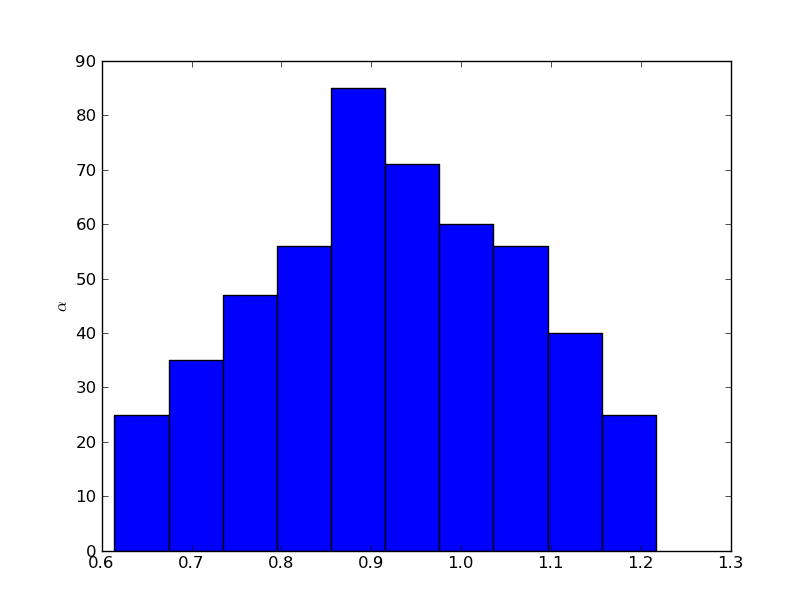
\includegraphics[width=0.5\linewidth]{rej_th1_lv.png}} 
   & \subfloat[]{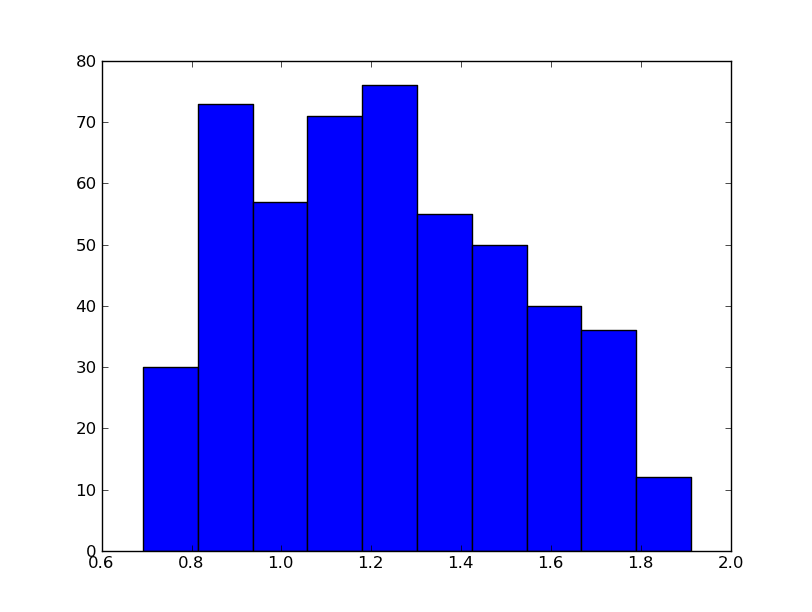
\includegraphics[width=0.5\linewidth]{rej_th2_lv.png}}\\
\multicolumn{2}{c}{\subfloat[]{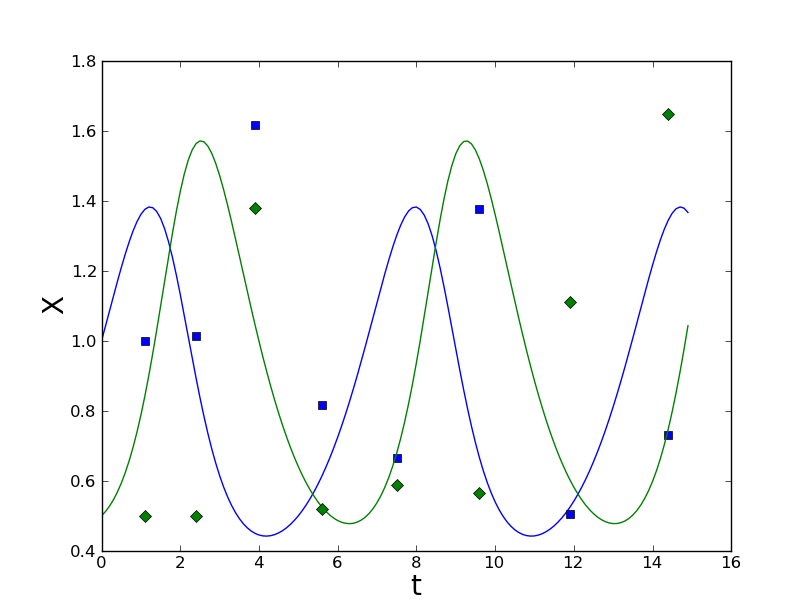
\includegraphics[width=0.5\linewidth]{realSim_rej_lv.png}} }
 
\end{tabular}
\end{tabularx}
\caption{Results for different values of parameter $\lambda$}\label{fig:solution_rej_lv}
\end{figure}
Then we applied the MCMC algorithm. We used a proposal distribution to generate candidate parameter vectors $\theta^*$  centred around the previous accepted value in the chain $\approx \mathcal{N}(\theta_i, \sigma)$. The normal proposal distribution was adaptive with its variance $\sigma$ being initially large $\sigma = 5$. Once a particle is accepted the variance is decreased to $0.1$. The rejection counter is set to $50$ and if that is reached the variance is increased again to $5$. In order to accept $500$ particles we need approximately $10000$ to $30000$ simulation steps. This is around 5 times less simulation steps than the simple rejections sampler which is expected since we minimise the samples taken from areas of parameter space with low likelihood and make a more informed search. The results however are similar to the results obtained with the previous method, $a$:median=$$, interquartile range=$$, $b$:median=, interquartile range=
\subsubsection{Parameter inference for repressilator model}
To test the implemented SMC algorithm we turn into a molecular biology example, the repressilator model which was purposefully chosen to highlight some of the challenges associated with parameter estimation and also the utility of the information gathered from ABC algorithms. The repressilator model\cite{garcia2004modeling} is a popular synthetic gene regulatory network. It consists of three genes connected in a feedback loop and each of the genes transcribes for a protein that represses the next gene in the loop with the last one repressing the first(Figure\ref{fig:repressilator}). The evolution of the concentrations of the mRNA products and their corresponding proteins can be written as a system of ODEs,
\begin{equation}
\begin{array}{lcl}
\dot m_1 & = & -m1 + \frac{\alpha}{1 + p_{3}^{n}} + \alpha_0 \\
\dot p_1& = & -\beta(p_1 - m_1) \\
\dot m_2 & = & -m2 + \frac{\alpha}{1 + p_{1}^{n}} + \alpha_0 \\
\dot p_2 & = & -\beta(p_2 - m_2)\\
\dot m_3 & = & -m3 + \frac{\alpha}{1 + p_{2}^{n}} + \alpha_0 \\
\dot p_3 & = & -\beta(p_3 - m_3),
\end{array}
\end{equation} 
\begin{figure}
\centering
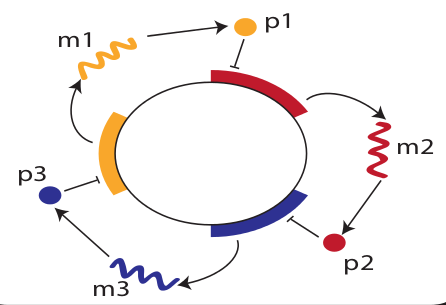
\includegraphics[width=0.5\linewidth]{repressilator}
\caption{The repressilator model. Three genes connected in a feedback loop where the protein product of each gene represses the production of the next gene in the loop.}
\label{fig:repressilator}
\end{figure}
where $m_i$ denotes the mRNA concentration and $p_i$ the corresponding protein one.  The model is parameterised by parameter vector $\theta = (\alpha, \alpha_0, \beta, n)$ where $n$ is the Hill coefficient, $\alpha$ the repression strength, $\beta$ the ratio of the protein decay rate to the mRNA decay rate and $a_0$ the basal expression rate. 

We assume that only the mRNA concentrations $\{m_i\}_1 \le i \le 3$ are known. We fix the parameter values at $(\alpha, \alpha_0, \beta, n) = (216.0, 0.216, 5.0, 2.0)$ and create a synthetic dataset consisting of the mRNA concentrations at timepoints taken at regular intervals in the range $[0, 50]$(for the exact dataset used see Appendix).
\subsection{Implementation details}
%starting talking a bit about software side..talk about the choice of python and the relative merits...talk about how the algorithms are implements and the structure of the code a bit
The language of choice for the implementation of the tool is Python. It is a highly extensible language leading to the development of a huge number of third party libraries for many tasks. There exist many scientific packages in Python like scipy\cite{scipy}, numpy with a large and lively community of users. It is also a free language therefore easily available making it a good choice for the development of tools that can be accessible to large user-base. Its use in systems biology is also increasing\cite{myers2007python, olivier2002modelling}.




%=======================================================================================================================================================================================================================
%=======================================================================================================================================================================================================================
%=======================================================================================================================================================================================================================



\section{System dynamics and infer-ability}
In this section we take a more theoretical approach to parameter estimation and investigate how the global dynamics of the system affect the parameter inference process. The qualitative structure of the solutions of dynamic systems can change as their parameter are varied. These qualitative changes in the dynamics are called bifurcations and the parameter values at which they happen are called bifurcation points. There are different kinds of bifurcations depending on different changes in the dynamics of the system. Here we are concerned with bifurcations that give rise to limit cycles in the phase plane of the solutions and therefore are capable of producing oscillatory behaviour.  Oscillators are present in many biological systems: cell cycles, circadian rhythms, calcium oscillations, pace maker cells, protein responses. Their behaviour in theoretical models is often captured through limit cycle oscillators which are driven by different kinds of bifurcations. In this section we will investigate two bifurcation capable of creating/destroying limit cycles in two-dimensional systems, Hopf Bifurcation and Saddle-Node bifurcation of Invariant Cycle(SNIC). Systems driven by these bifurcations have been used for real and synthetic oscillatory systems in biology. Their dynamics have also been contrasted in designs of the same synthetic genetic oscillator logical motif\cite{guantes2006dynamical}.  Since models that use these kinds of bifurcations are used extensively in biology, it is of value to investigate the challenges associated with parameter estimation in those types of models.

In Hopf Bifurcation as the control parameter passes through the bifurcation point, a fixed point of the system loses its stability and the systems shows a limit cycle around that fixed point. In general before the bifurcation point, when the system is temporally perturbed we have damped oscillations which decay and settle down to an equilibrium state(stable fixed point). However in the presence of noise the perturbations are constant and the system does not settle down and therefore it been shown that sustained oscillations can be produced albeit with fluctuating amplitude. After the value of the control parameter passes through the bifurcation point the fixed point loses its stability, a limit cycle is formed around the fixed point and the systems shows sustained oscillations.  Both mechanisms, limit-cycle oscillator with unstable fixed point and noise-induced oscillator with stable fixed point, have been proposed as a driving force for oscillatory systems.

In SNIC bifurcation a limit cycle appears as  fixed points are created from nothing when the control parameter passes through the bifurcation point. In this case however the stability of the fixed point does not change.

\subsection{Methods}
\subsubsection{Models}
For our investigation of the effects of a Hopf bifurcation we chose a very simple system that undergoes a Hopf bifurcation\cite[p.250] {strogatz2001nonlinear}. The simplicity of the model is convenient for our investigation while still maintaining the relevant characteristics. The system given in polar coordinates,
\begin{equation}
\begin{array}{lcl}
\dot r &= & \mu r -r^3 \\
\dot \theta &= & \omega + b r^2.
\end{array}
\end{equation}
The system has three parameters: $\mu, \omega, b$. The control parameter for the bifurcation is $\mu$ so we consider the other two known, $(\omega, b)=(1,1)$ and investigate the behaviour as $\mu$ varies. The system has a fixed point $(0,0)$ which undergoes a Hopf Bifurcation losing its stability as the control parameter $\mu$ goes through $0$.

For our investigation of the effects of the SNIC bifurcation we again chose a very simple system\cite[p.250] {strogatz2001nonlinear}. The system in polar coordinates,
\begin{equation}
\begin{array}{lcl}
\dot r &= & \mu r +r^3 - r^5 \\
\dot \theta &= & \omega + b r^2.
\end{array}
\end{equation}
The control parameter for the bifurcation is $\mu$. The radial equation $\dot r =  \mu r +r^3 - r^5$ undergoes a saddle-node bifurcation of fixed points at $\mu=-1/4$ and two new fixed points are created. When view in the two-dimensional setting these correspond to the creation of limit cycles.
\subsubsection{Maximum Likelihood for ODEs}
\label{sec:likelihood}
For any mathematical model our goal is to infer true parameters $\theta^*$ given some observed data $\mathbf{Y_{d}} =\{\mathbf{y_{t_1}}, \mathbf{y_{t_2}}, \dots, \mathbf{y_{t_M}}\}$ at times $\{t_{i}\}_{1 \le i \le M}$. To this end we wish to know the likelihood function $L(\theta | \mathbf{Y_{d}})$ which tells us how the probability of observing the data $\mathbf{Y_{d}}$ changes with $\theta$. However, a direct approach to obtaining the likelihood function is not possible for deterministic system of ODEs but subject to some assumptions the likelihood function is equivalent to the distance or error between real(observed) and predicted data. That means that the probability of observing the data $\mathbf{Y_{d}}$ for parameter vector $\theta_{s}$ is equivalent to $\Delta(\mathbf{Y_{d}}, \mathbf{Y_{\theta_s}})$ where $\mathbf{Y_{d}}$ is the real data,$\mathbf{Y_{d}}$ data simulated with parameter $\theta_{s}$ and $\Delta$ is the Euclidean distance. This is also the intuition behind using comparisons of real and simulated data with the Euclidean distance as an approximation for the Likelihood function in the ABC algorithms. 

Here we follow the likelihood approach for ODE parameter estimation given in \cite{}. We assume that any observed data point $\mathbf{y_{t_i}}$ is distributed according to $\mathcal{N}(\boldsymbol{\mu}_{t_i}(\theta), \Sigma_{t_i})$, where $\boldsymbol{\mu}_{t_i}(\theta)$ is the solution of the system $\dot x = \mathbf{F}(\mathbf{x}, t, \theta)$ at time $t_i$ and $\Sigma_i$ is a covariance matrix which is the same for all $i$. Then the likelihood function is given by:
\begin{equation}
L(\theta | \mathbf{Y_d}) = \prod_{i=1}^M \frac{1}{(2\pi)^{3/2}|\Sigma|^{1/2}} \exp \left(-\frac{1}{2}(\mathbf{y_{t_i}} - \mu_i(\theta))^{T}\Sigma^{-1}(\mathbf{y_{t_i}} - \mu_i(\theta)) \right).
\end{equation}
We will investigate the behaviour through the log-likelihood function,
\begin{equation}
\begin{array}{lcl}
ln(L(\theta|\mathbf{Y_d}) &= & M ln\left(\frac{1}{(2\pi)^{3/2}|\Sigma|^{1/2}}\right) -\frac{1}{2}\sum_{i=1}^{M}((\mathbf{y_{t_i}} - \mu_i(\theta))^{T}\Sigma^{-1}(\mathbf{y_{t_i}} - \mu_i(\theta))\\
& \propto & -\frac{1}{2}\sum_{i=1}^{M}(d_{\Sigma}(\mathbf{y_i} - \boldsymbol{\mu_i(\theta)}))^2,
\end{array}
\end{equation}
where $d_{\Sigma}(\mathbf{y_i} - \boldsymbol{\mu_i(\theta)}) = \sqrt{(\mathbf{y_{t_i}} - \mu_i(\theta))^{T}\Sigma^{-1}(\mathbf{y_{t_i}} - \mu_i(\theta)}$ is the Mahalanobis distance between $\mathbf{y_{t_i}}$ and $\boldsymbol{\mu_i(\theta)}$ with respect to $\Sigma$.  Subject to our assumption that the covariance matrix $\Sigma$ is equal for $i$ then the Mahalanobis distance is equivalent to Euclidean distance and the log-likelihood function is given by,
\begin{equation}
ln(L(\theta|\mathbf{Y_d}) = -\frac{1}{2}\sum_{i=1}^{M}(d(\mathbf{y_{t_i}}, \mu_{i}(\theta)))^2,
\end{equation}
where $d(\mathbf{y_{t_i}}, \mu_{i}(\theta))$ is the Euclidean distance between $\mathbf{y_{t_i}}$ and$\mu_{i}(\theta))$. It is clear that maximising the 
likelihood function is equivalent to minimising the distance function $d$. Obviously the maximum likelihood estimate will be at the value of the true parameter where real and simulated data are the same and the distance value is equal to $0$. Therefore this likelihood function is related to the problem of finding how far apart are solutions with the same initial conditions as the parameters vary. This is how the likelihood function is also related to the parameter inference process. The landscape of the likelihood function around the true parameter value can give some information on how easy the parameter estimation process will be. For example flat regions imply regions of highly likely values which are close to the true solution therefore suggesting high acceptance rates in the filtering process of ABC schemes. In the next section we investigate how the shape of the likelihood function and consequently the parameter estimation process changes as the systems undergo a bifurcation.

\subsection{Results}
%Hopf bifurcation=============================
\subsubsection{Hopf Bifurcation}
\begin{table}[ht]
\centering
\begin{tabular}{cc}
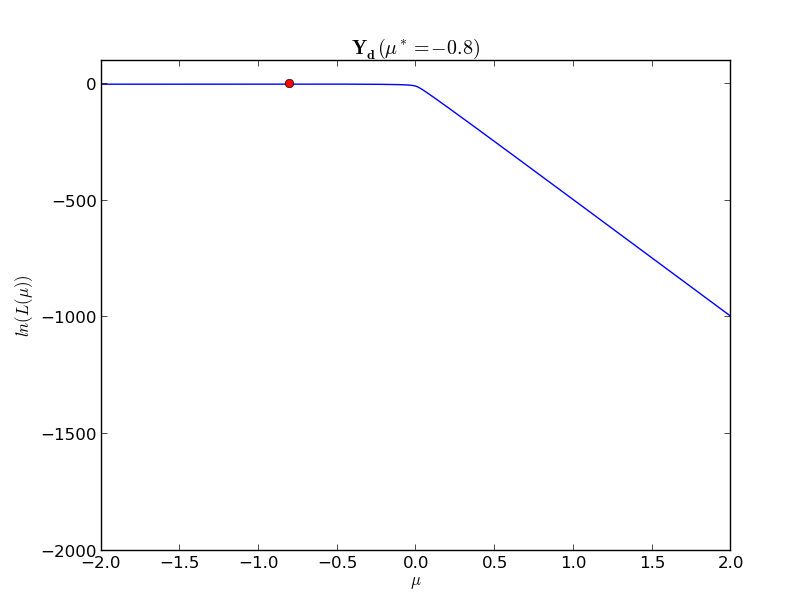
\includegraphics[scale=0.3]{likelihood_hopf08m}&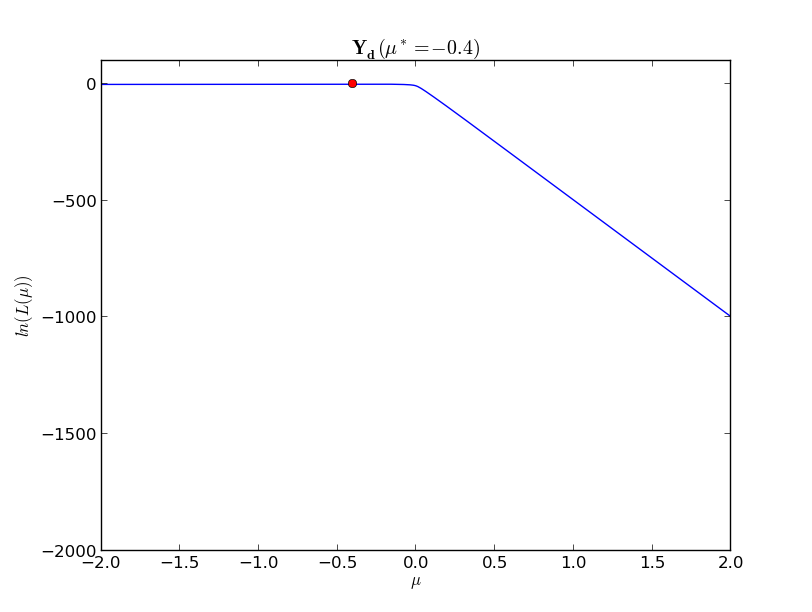
\includegraphics[scale=0.3]{likelihood_hopf04m}\\
\newline
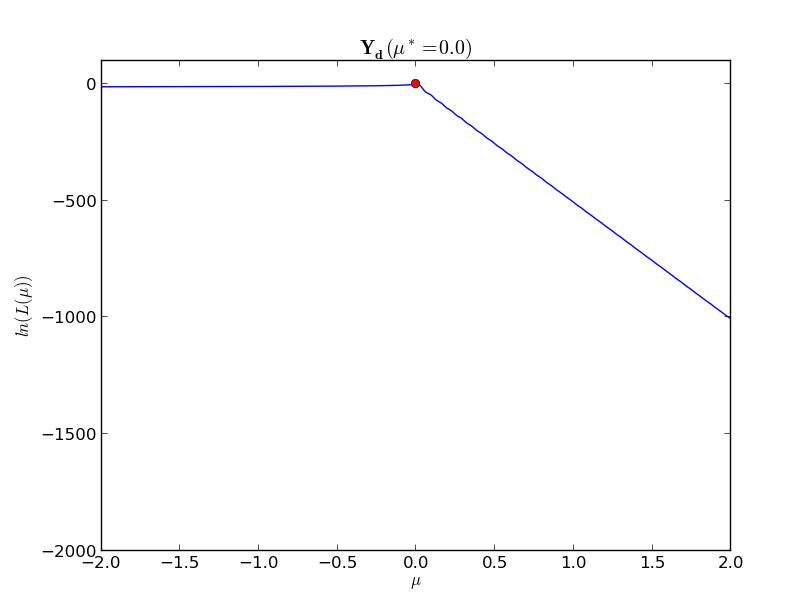
\includegraphics[scale=0.3]{likelihood_hopf0}&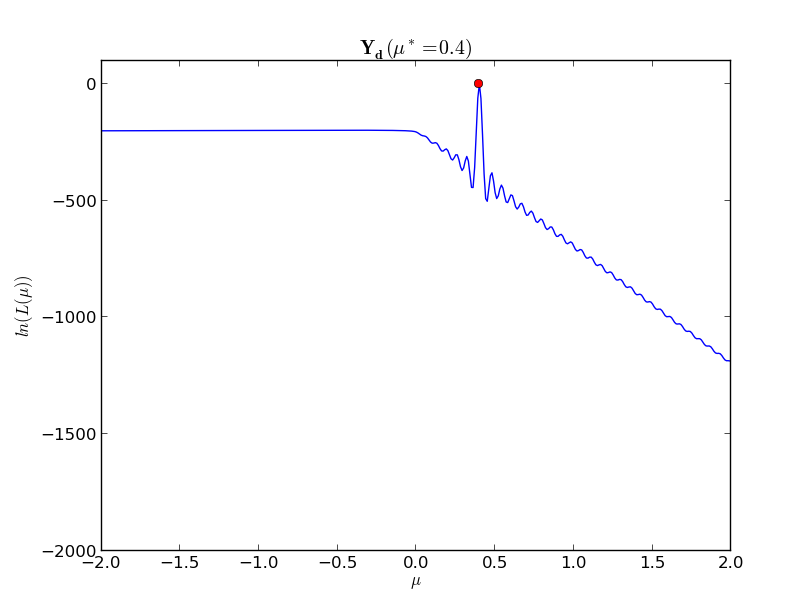
\includegraphics[scale=0.3]{likelihood_hopf04}\\
\newline
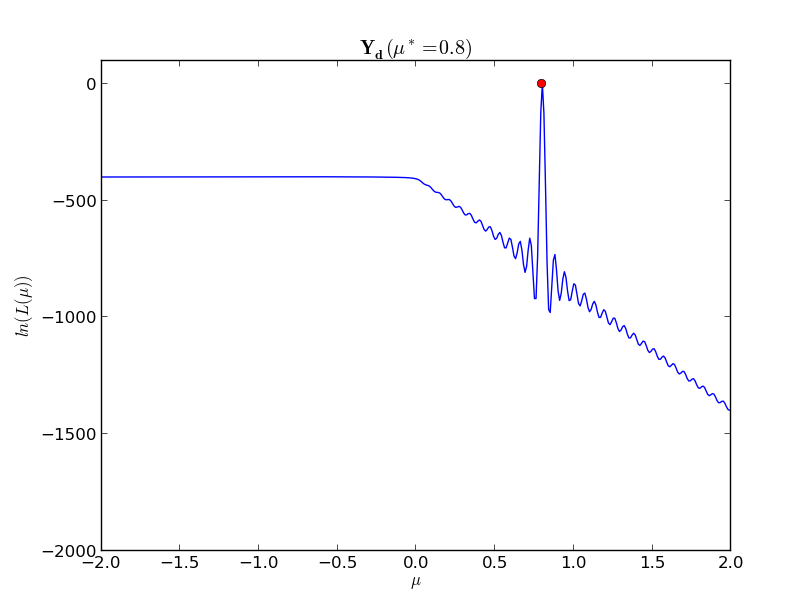
\includegraphics[scale=0.3]{likelihood_hopf08}&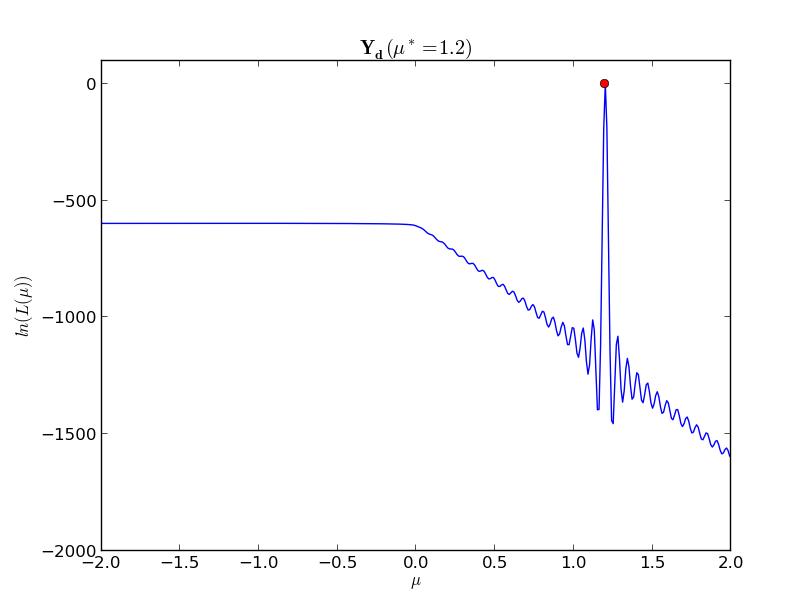
\includegraphics[scale=0.3]{likelihood_hopf12}\\
\end{tabular}
\caption{Log-likelihood plots for different values of $\mu^*$ specified in the header. The maximum likelihood is denoted by the red dot which is as expected at the true value.}
\label{fig:hopf}
\end{table}
To understand the effects of Hopf bifurcation we plot the log-likelihood function, $\text{ln}(L(\mu | \mathbf{Y_{d}}(\mu^*)))$ for parameter $\mu$ which is the control parameter for the bifurcation, for different values of $\mu^*$ both sides of the bifurcation point. The resulting plots are in \ref{fig:hopf}. As expected the maximum likelihood estimator is at the true value. However there is a big qualitative change in the shape of the log-likelihood functions when $\mu > 0$ and when $\mu < 0$. 

For the landscape of the log-likelihood plot for values $\mu^* < 0$ we observe a relatively flat region in the interval [-2.0, 0.0] and then a relatively steep part with negative gradient in the interval [0.0, 2.0]. The flat part in the region $-2 \le \mu \le 0$ tells us that parameter estimates in that domain are all highly likely.This is easy to understand as the corresponding solutions for estimates in that domain  are qualitatively similar to each other and to the solution for $\mu^*$. Therefore the distance between them and also between them and the solution for $\mu^*$ is small which is reflected on the likelihood plot. As the value of $\mu$ goes through the bifurcation point, the estimates become increasingly unlikely which can also be explained by the fact that the solutions corresponding to estimates in this domain are qualitatively very different from the solution for $\mu^*$. Moreover the bifurcation point at $\mu = 0$ which marks the point of change in system dynamics also marks the change in the behaviour and shape of the likelihood function.

For the landscape of the log-likelihood plot at the other side of the bifurcation for values $\mu^* > 0$ we observe the maximum likelihood estimate, as expected at the true value, but this occurs at a spike in the curve. That tells us that solutions that correspond to parameter estimates which are near the true value $\mu^*$ are not very likely so small changes in the control parameter near the true value $\mu^*$ result to big changes in the corresponding solution. Again the bifurcation point at $\mu=0$ is recognisable by the change in the behaviour of the graph at that point. Solutions for estimates in the region [-2, 0] are similar so their distances from the solution for true parameter value are similar, hence the flat part of the graph.On the other hand solutions corresponding to estimates in the region [0, 2] are relatively dissimilar, hence the bigger changes in the distances to the true solution we observe via a steeper descent in the graph in that region.

To understand the change in the distances between adjacent and solutions and the change in the shape of the likelihood function as the control parameter goes through the bifurcation point we can look at what happens to the system dynamics. This will be easier if we look at solutions as trajectories in the phase plane\ref{fig:phase_plane_hopf}. At one side of the bifurcation point for values of $\mu^* < 0$ the fixed point of the system is stable therefore trajectories near the fixed point will get attracted to it. This makes solutions for nearby parameter estimates in that region qualitatively very similar which makes the distance between them very small. Given the equivalence of distance with likelihood, we expect estimates in that region to be highly likely which is verified by our findings. When the control parameter passes through the bifurcation point, the fixed point of the system becomes unstable therefore trajectories that start near it will be pushed away from it towards the limit cycle around it. This makes solutions that start from the same initial conditions more dissimilar and the distance between them higher. In order to approach the observed data for $\mu^*$ the parameter estimate will have to be close to it.
\begin{table}[ht]
\centering
\begin{tabular}{cc}
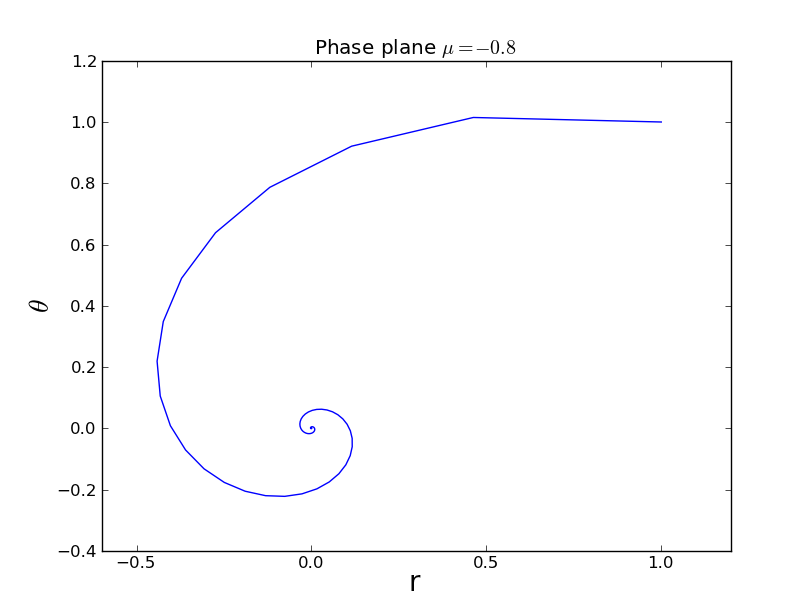
\includegraphics[scale=0.3]{phase_hopf08m}&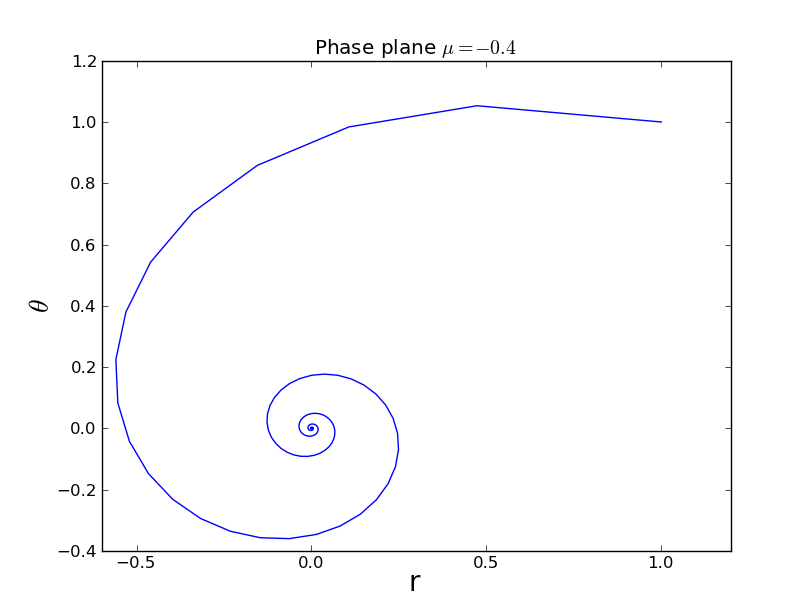
\includegraphics[scale=0.3]{phase_hopf04m}\\
\newline
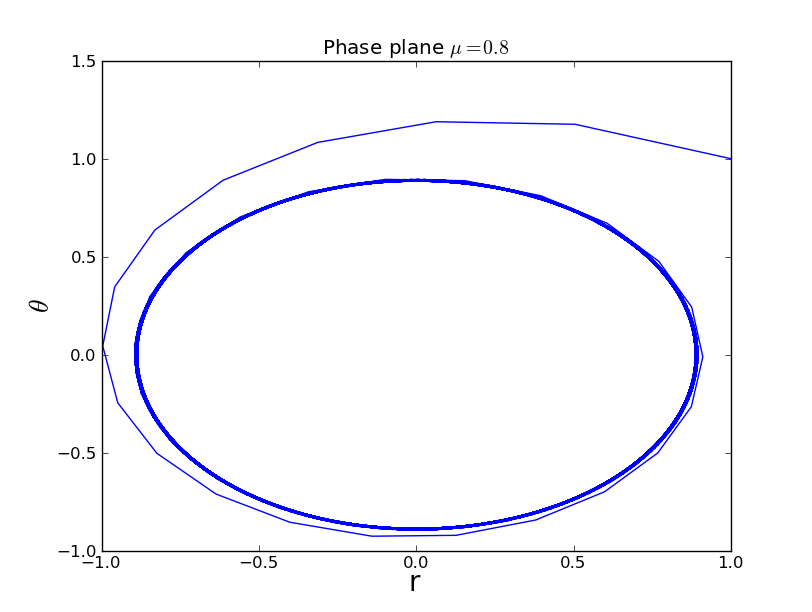
\includegraphics[scale=0.3]{phase_hopf08}&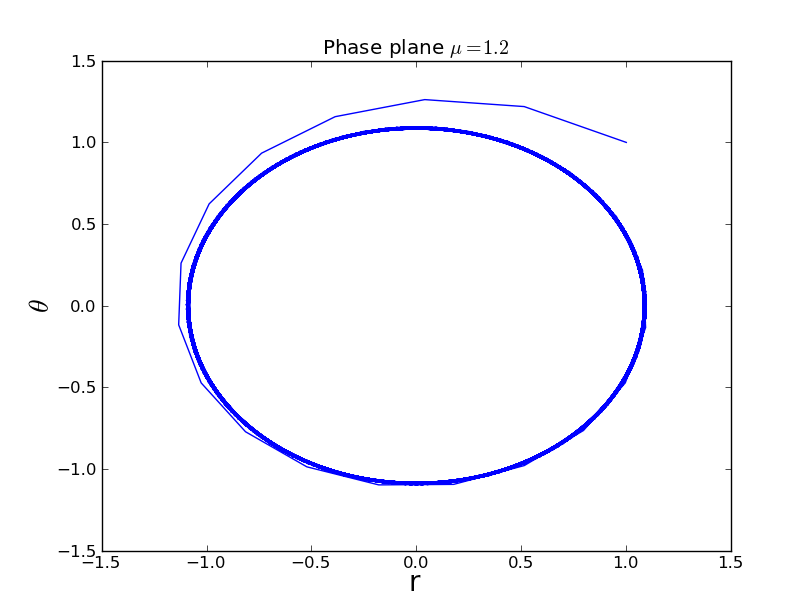
\includegraphics[scale=0.3]{phase_hopf12}\\
\end{tabular}
\caption{Solutions corresponding to trajectories in the phase plane for different value of
control parameter $\mu$ either side of the bifurcation point $\mu = 0$.}
\label{fig:phase_plane_hopf}
\end{table}

The connection between the shape of the likelihood function and the distance between nearby solutions and the practicalities of the parameter inference process should be apparent. For values $\mu^* < 0$ nearby solutions are similar so we expect a high acceptance rate and less iteration steps at the filtering steps of ABC schemes that use the distance function as a filter. The population obtained from the ABC scheme however will be spread out(high variance) which might decrease the confidence for the estimate. On the other hand from the other side of the bifurcation point and for values $\mu^* > 0$ where nearby solutions are not very similar we expect a lower acceptance rate and more iterations steps. But we expect the obtained population to be more concentrated giving a higher confidence for the estimate. These are indeed verified as we test the SMC scheme for%give resutls

There is a also an apparent link between the shape of the likelihood function and parameter sensitivity. A spike in the log-likelihood curve tells us that a the system is very sensitive to changes in that parameter. Small changes in the parameter value get amplified in the solution. On the other hand a relatively flat region around the true parameter value tells us that the model is not very sensitive to that parameter as changes to it result in small changes in the corresponding solutions. Hence this is another way to see the importance of the rich information obtained from ABC schemes. ABC schemes return a distribution for the parameter estimate instead of a single value. As we have seen populations of parameter estimates that are concentrated around a specific value with low variance imply low likelihood estimates around the true parameter. This can be translated to a spike in the shape of the log-likelihood function, for example in \ref{} and therefore to high sensitivity of the system to that parameter. Populations of parameter estimates which are more spread out with high variance imply highly likely estimates around the true parameter value and hence a flat region of the likelihood function which tells us that the system is not very sensitive to that parameter.


\subsubsection{SNIC}
\begin{table}[ht]
\centering
\begin{tabular}{cc}
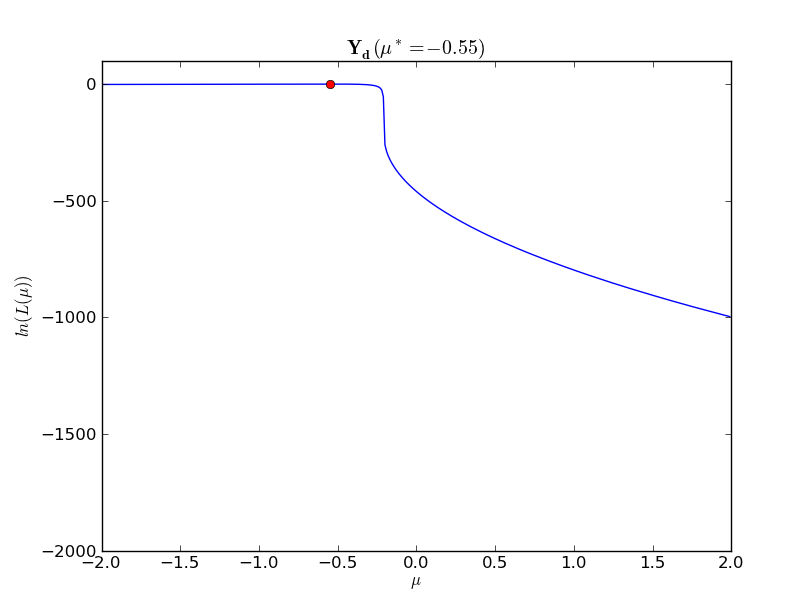
\includegraphics[scale=0.3]{likelihood_sinc_055m}&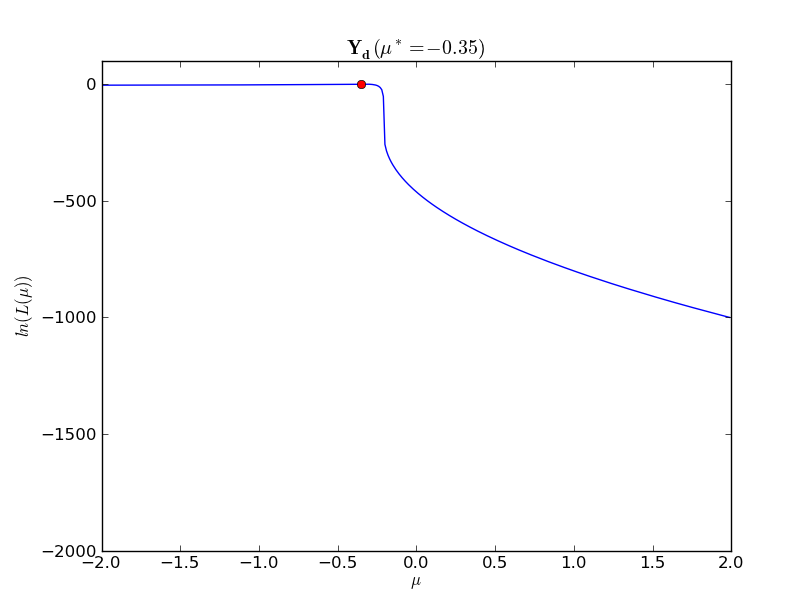
\includegraphics[scale=0.3]{likelihood_snic035m}\\
\newline
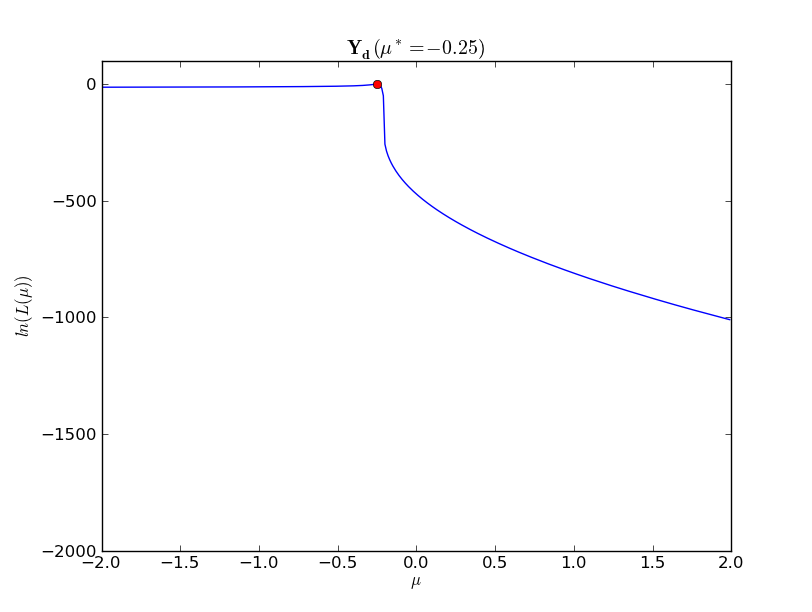
\includegraphics[scale=0.3]{likelihood_snic025m}&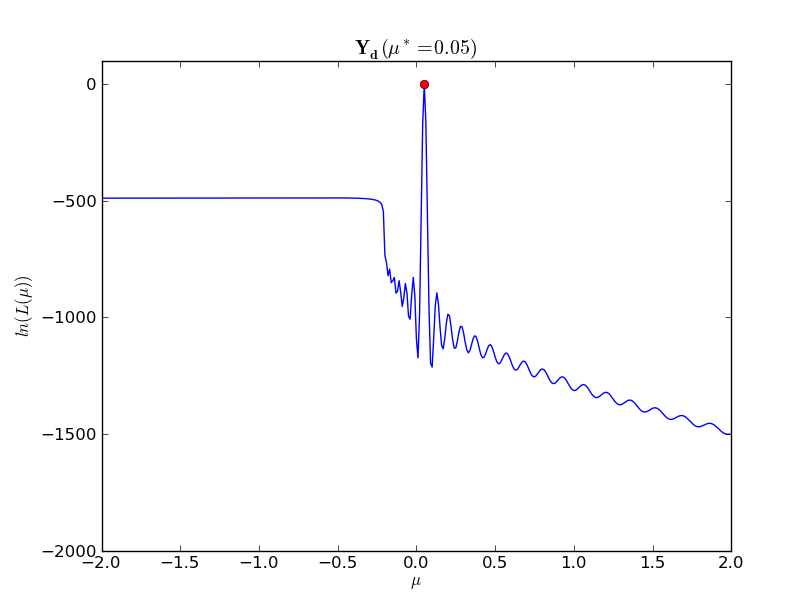
\includegraphics[scale=0.3]{likelihood_snic005}\\
\newline
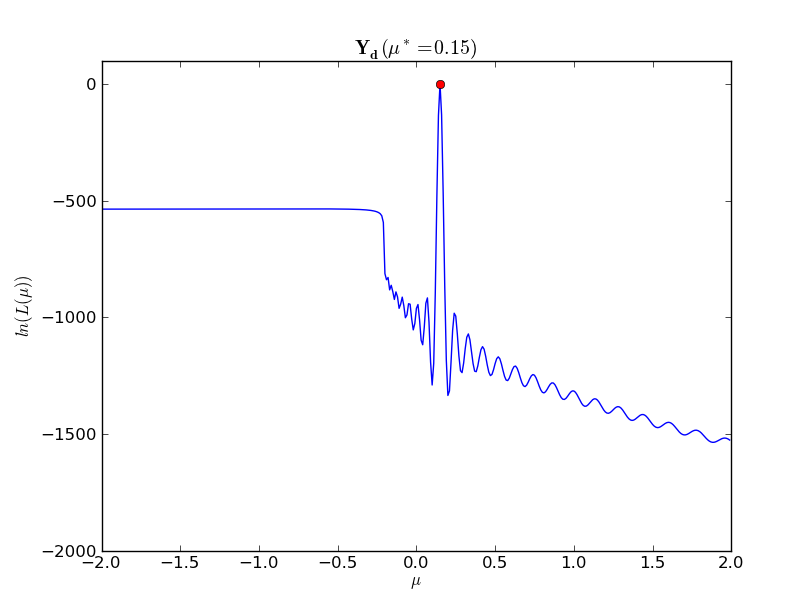
\includegraphics[scale=0.3]{likelihood_snic015}
\end{tabular}
\caption{Log-likelihood plots for different values of $\mu^*$ specified in the header. The maximum likelihood is denoted by the red dot which is as expected at the true value.}
\label{fig:snic}
\end{table}
We proceed to investigate the effects of the SNIC bifurcation in the same way as we have for the the Hopf bifurcation. We plot the likelihood function $\text{ln}(L(\mu | \mathbf{Y_{d}}(\mu^*)))$ for values of $\mu^*$ either side of the bifurcation point at $\mu = -1/4$ for a range of values of $\mu$ in the range [-2, 2] taken at regular intervals of $0.01$. The resulting log-likelihood plot are in Figure\ref{snic}. As expected the maximum likelihood estimator is always at the true value $\mu^*$, however we again notice a qualitative change in the plots either side of the bifurcation point.

For the landscape of the plots of log-likelihood functions for values of parameter before the bifurcation point $\mu^* < -1/4$ there is flat region in the area from [-2, -1/4], then an elbow in the curve at the bifurcation point and then a steeper area with negative gradient. This is qualitatively the same as the log-likelihood functions at one side of the Hopf bifurcation point in the previous section. The flat part tells us that solutions in that range are all relatively close to the true solution and the steep part that solutions in that area become increasingly unlikely. Again this change is due to the change in the system dynamics either side of the bifurcation point.

For the landscape of the plots of log-likelihood function for values of parameter after the bifurcation again we get similar results as in the Hopf bifurcation case when the limit cycle appears in the phase plane. The maximum likelihood estimate at the true value happens as a spike in the curve which tells us that nearby estimates are unlikely so solutions that start at the same initial condition vary considerably as the parameters change. 
\begin{table}[ht]
\centering
\begin{tabular}{cc}
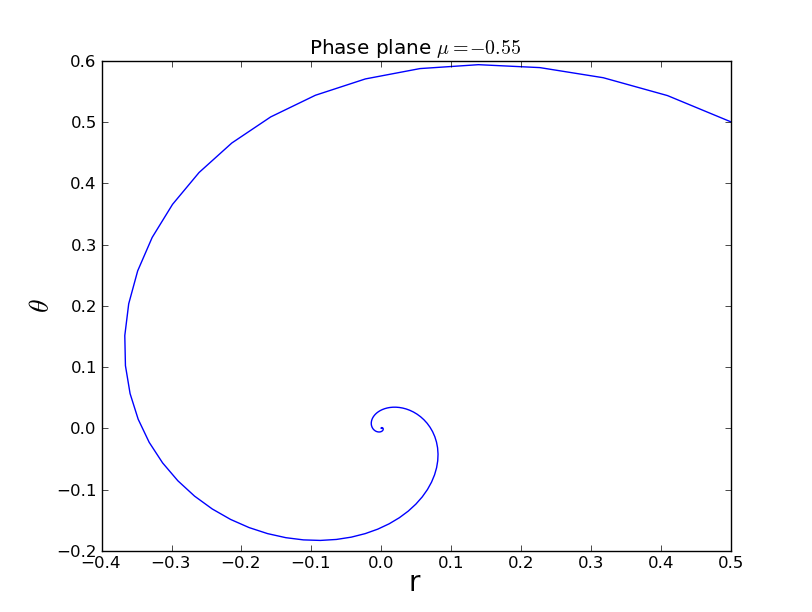
\includegraphics[scale=0.3]{phase_snic055m}&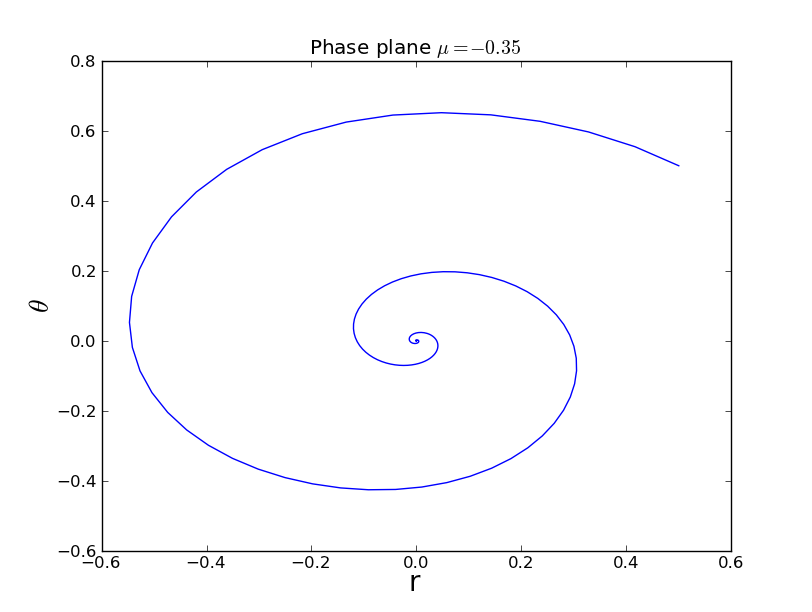
\includegraphics[scale=0.3]{phase_snic035m}\\
\newline
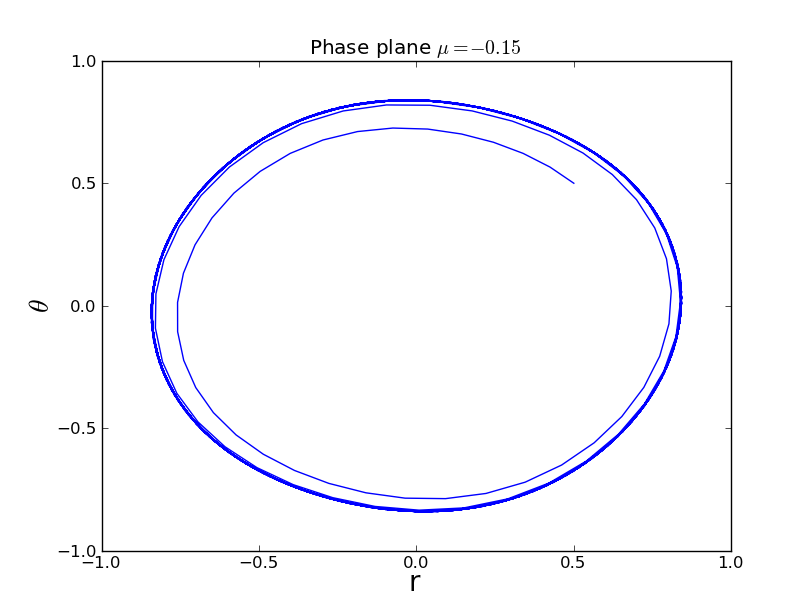
\includegraphics[scale=0.3]{phase_snic015m}&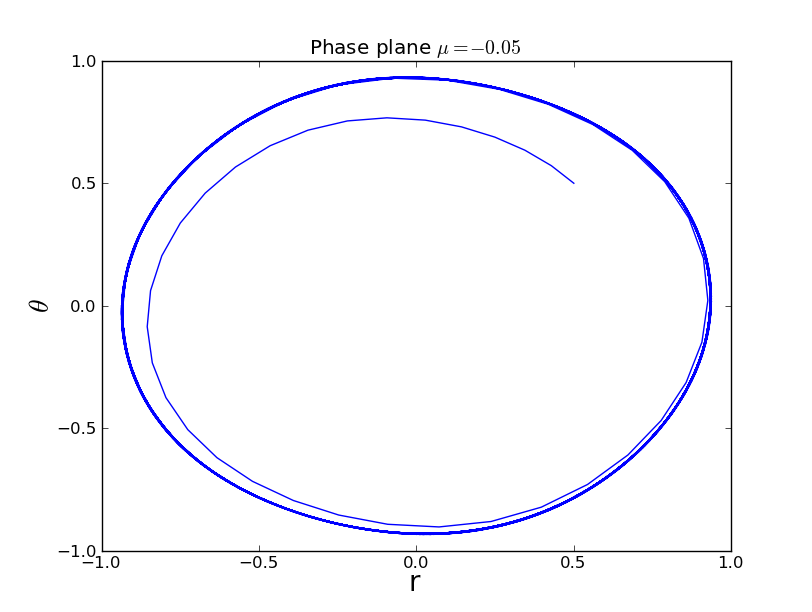
\includegraphics[scale=0.3]{phase_snic005m}\\
\end{tabular}
\caption{Solutions corresponding to trajectories in the phase plane for different value of
control parameter $\mu$ either side of the bifurcation point $\mu = 0$.}
\label{fig:phase_plane_hopf}
\end{table}
The findings can again be explained by the change to the system dynamics as the system undergoes the bifurcation and to the corresponding solutions as trajectories in the phase plane. For values of the control parameter before the bifurcation point $\mu < -1/4$ the fixed points in the radial equation annihilate each other as it undergoes a saddle-node bifurcation and the limit cycles are destroyed. The fixed point is stable though so trajectories starting near it will get drawn towards it. In that way solutions resemble solutions of the Hopf bifurcation system before the bifurcation point. Because solutions get drawn towards the fixed point which makes solution for different parameter values qualitatively very similar hence the flat part in the region. After the control parameter goes through the bifurcation point at $\mu=-1/4$ the fixed point does not lose its stability as in the Hopf bifurcation case but two fixed points appear in the radial equation which correspond to limit cycles in the two-dimensional case. Therefore solutions that start near that fixed point will get pushed out to the limit cycle which is the same kind of behaviour that we get from the Hopf bifurcating system in the previous section. Nearby solutions will be qualitatively not very similar unless their corresponding control parameter values are really close hence the spike in the log-likelihood curves for $\mu > -1/4$.

So we have found that the two bifurcation that can create limit cycles in the two-dimensional case behave similarly as limit cycles are created even though the mechanism for their creation is not the same. 

%
%link the shape of the likelihhod function with parameter estimation process, get practical results...choose a system ...graph the likelihhood function both sites of a bifurcation point etc. etc., do a 2 parameter likelihhood surface plot as well




%=======================================================================================================================================================================================================================
%=======================================================================================================================================================================================================================
%=======================================================================================================================================================================================================================



\section{Discussion and Future Work}

\newpage
\bibliography{report}
\end{document}